\section{Arquitetura IoT, Comunicação e Dados}

A Figura~\ref{fig:sintese_arquitetura} sintetiza os enlaces entre os \ac{FAR} e a plataforma terrestre, a interface do operador e a gestão remota da infraestrutura~\cite{reeuwijk2025,oliveira2023tevel}.

\begin{figure}[!htb]
    \centering
    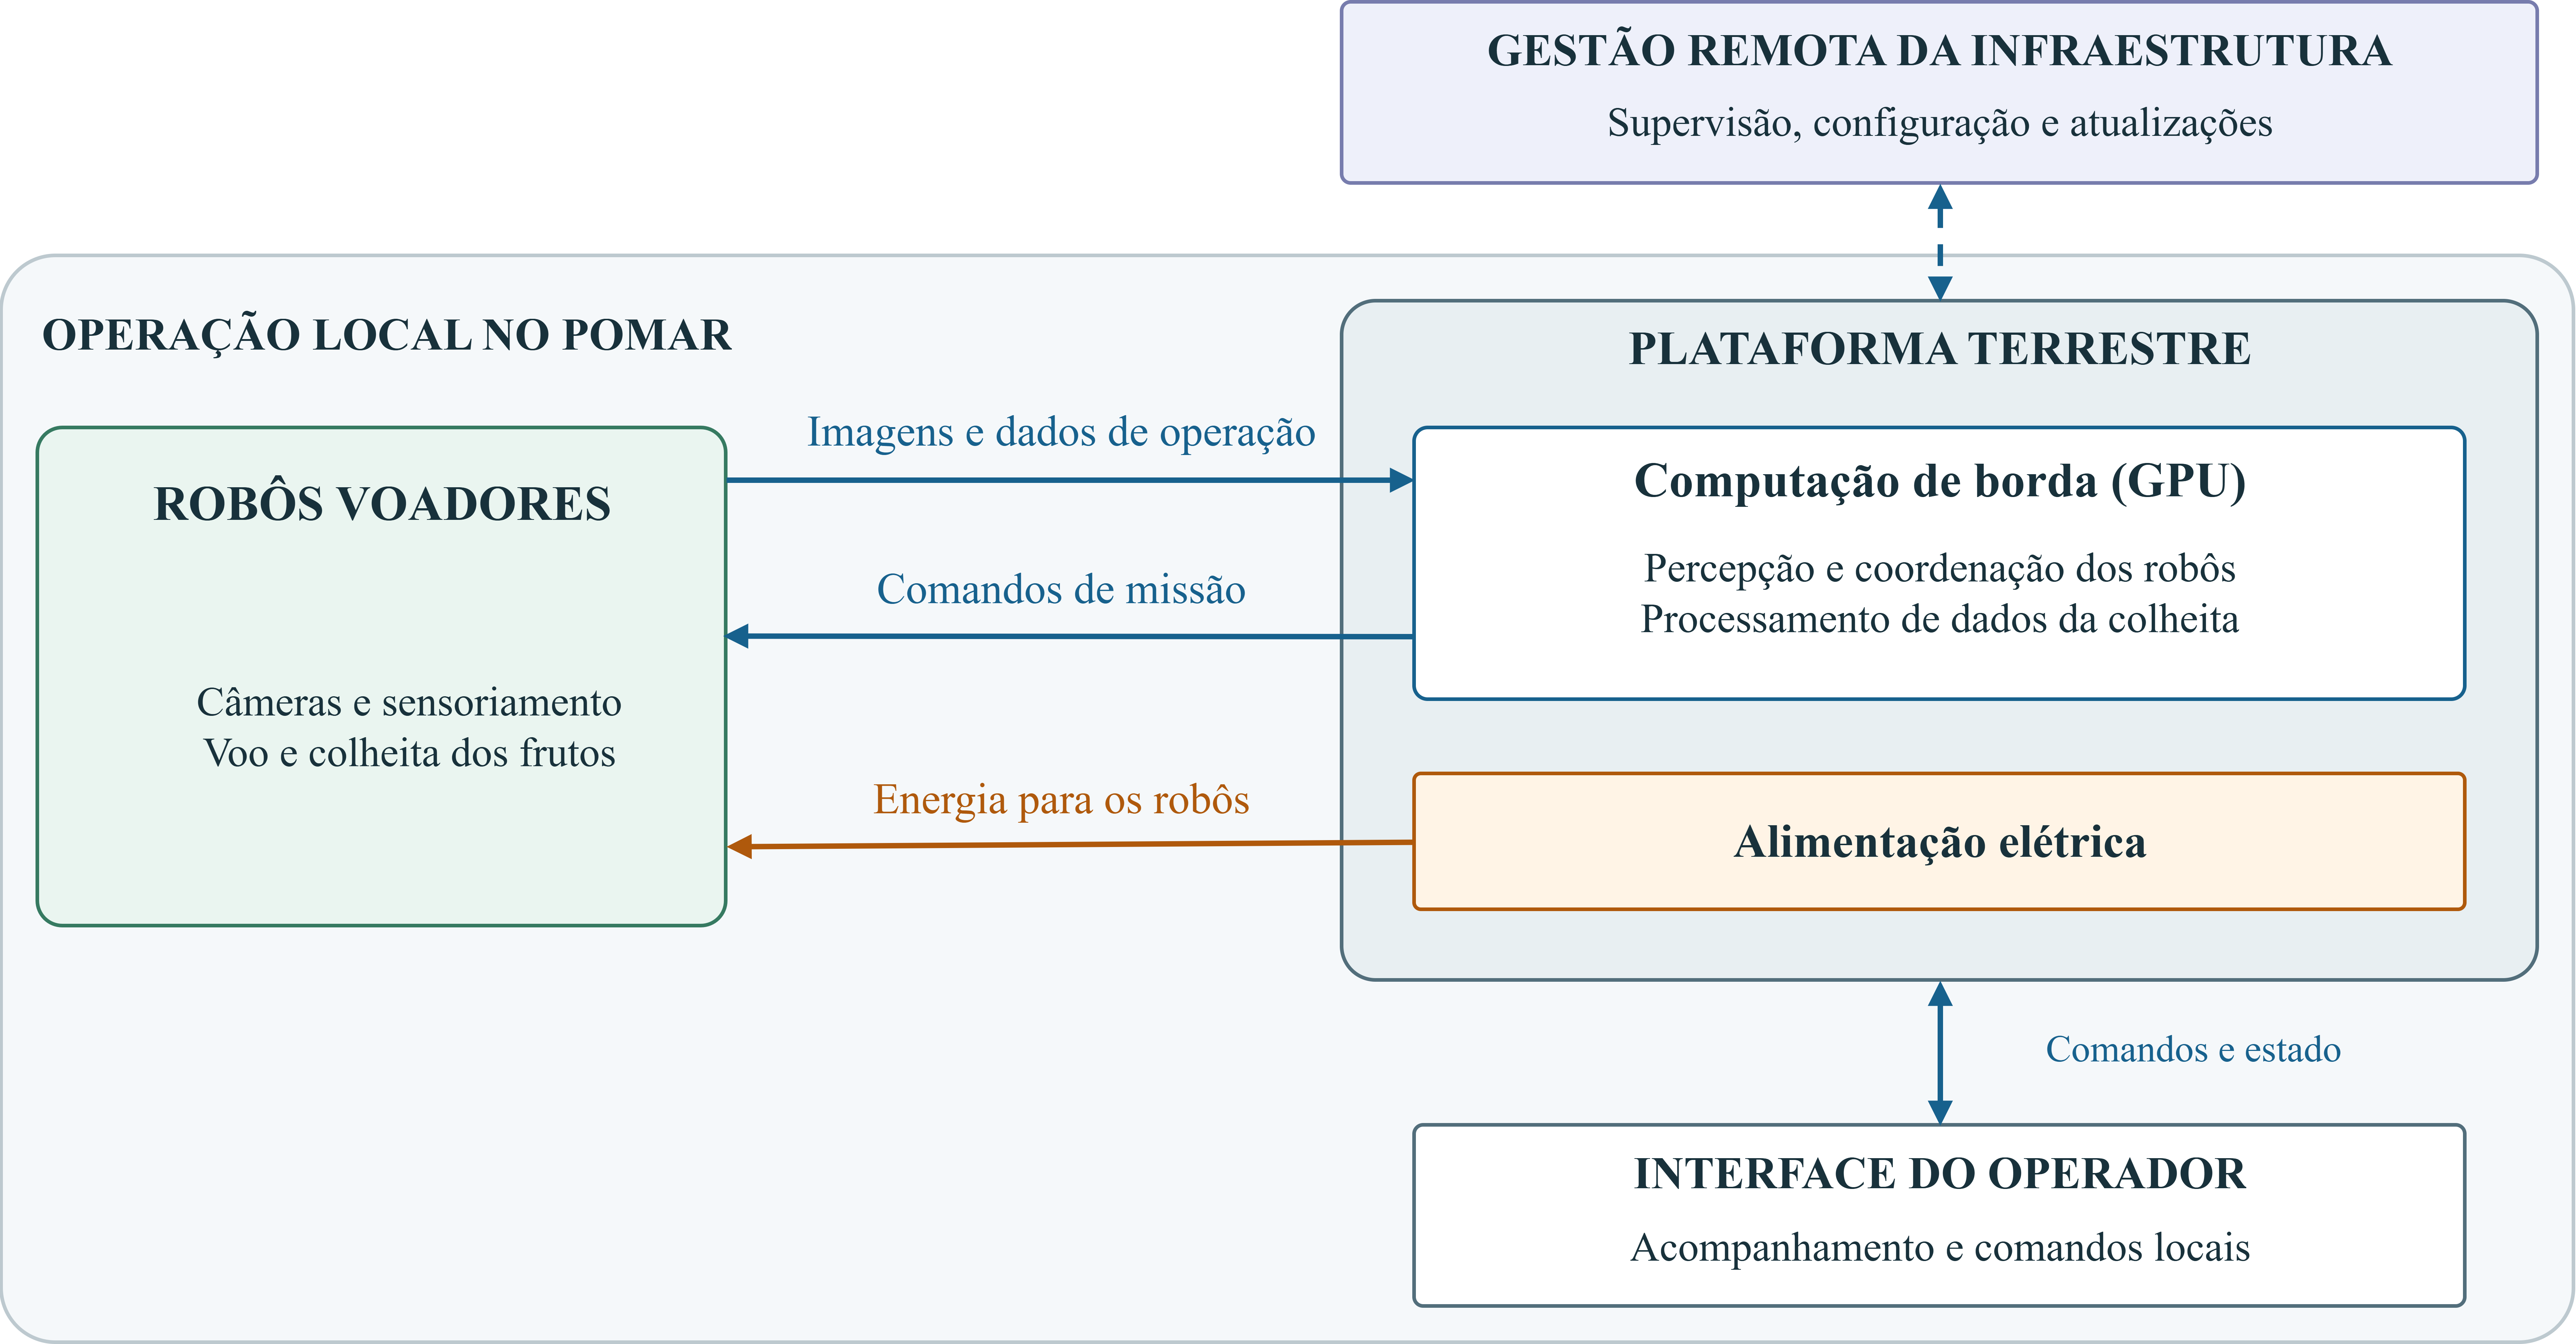
\includegraphics[width=0.98\linewidth]{figures/arquitetura_tevel.drawio.png}
    \caption{Síntese funcional da arquitetura.}
    \label{fig:sintese_arquitetura}
\end{figure}

Na apresentação de 2023, Tevel e Spectro Cloud destacam conectividade instável, dificuldade de acesso às instalações e operação durante desconexões. O material distingue a gestão remota dos ambientes de borda e apresenta a operação desconectada como requisito~\cite{oliveira2023tevel}. Essa organização visa manter as aplicações locais em execução quando a gestão remota estiver indisponível.

Esse requisito não demonstra tolerância à ruptura do cabo, à perda de alimentação ou à falha do computador terrestre, cujas respostas não são especificadas nas fontes consultadas. Tampouco se apresenta uma descrição completa dos protocolos entre robôs, estação e infraestrutura externa. Sem confirmação documental, não se atribuem ao produto \ac{MQTT}, LoRaWAN, 5G ou Ethernet.

A Tevel declara disponibilizar quantidade colhida, peso e tamanho dos frutos, classificação por cor, detecção de doenças, horário, geolocalização e distribuições de peso, tamanho e cor por recipiente~\cite{tevelTechnology}. Esses registros associam os frutos à sua representação digital e informam ao produtor a composição da colheita antes do beneficiamento.

A utilidade dos dados depende de rastreabilidade e qualidade. Sua avaliação exige distinguir medições de estimativas por visão, registrar falhas de aquisição e verificar a exatidão das classificações. As fontes consultadas não detalham todos os sensores, a calibração, a incerteza do peso ou a acurácia da detecção de doenças. A funcionalidade anunciada, portanto, não comprova desempenho metrológico ou diagnóstico validado.